\documentclass[]{article}
\newcommand{\FileDepth}{../../..}
\usepackage[letterpaper, landscape, margin=0.5cm]{geometry}
\usepackage[T1]{fontenc}
\usepackage{textcomp}%Not strictly necessary, but gives \textmu command for "micro."
\usepackage{fancyhdr}
\usepackage{amsmath}
\usepackage{amssymb}
\usepackage{graphicx}
\usepackage{xcolor}
\usepackage{tikz}
\usetikzlibrary{calc}
\usepackage[shortlabels]{enumitem}
\usepackage{multicol}
\usepackage{vwcol}
\usepackage{hyperref}
\usepackage{wrapfig}
%opening
\newcommand{\SecType}{S}
\newcommand{\Week}{3}
\title{PH 211 Studio \Week}
\author{Benjamin Bauml}
\date{Summer 2024}

\newcommand{\Purpose}{4}
\newcommand{\DefOnly}{0}

% Version 2024-06-14
% Changes
% 2024-02-21 Added xstring package to enable smooth implementation of new \ModePage command.
% 2024-04-27 Set up to split activities and formatting aspects into separate files. Removed dependence on xcomment. Added an automatic counter to number the activities in a problem set.
% 2024-05-19 Revised old format for \TeachingTips command, which did not support \DefOnly.
% 2024-06-14 Added Repurpose environment to allow mixing of different purpose levels in the same document.
\usepackage{tcolorbox}
\usepackage{xstring}
% You will want the following four lines in your document (the last two uncommented):
% For Assignment, leave Purpose as 1. For Worksheet, set to 2. For Student Solution, set to 3. For Teacher Solution, set to 4.
% If you want keep the pieces from being called manually, set DefOnly to 0.
%\newcommand{\Purpose}{4}
%\newcommand{\DefOnly}{1}
\newcommand{\Exclusion}{0}
\newcommand{\PageTurn}{0}
\newcommand{\GrayProb}{0}
\newcommand{\Tipsy}{0}

% Assignment
\if\Purpose1
\renewcommand{\Exclusion}{1}
\fi
% Worksheet
\if\Purpose2
\renewcommand{\Exclusion}{1}
\renewcommand{\PageTurn}{1}
\fi
% Student Solution
\if\Purpose3
\renewcommand{\PageTurn}{1}
\renewcommand{\GrayProb}{1}
\fi
% Teaching Copy
\if\Purpose4
\renewcommand{\PageTurn}{1}
\renewcommand{\GrayProb}{1}
\renewcommand{\Tipsy}{1}
\fi

\newenvironment{Repurpose}[1]{
\renewcommand{\Purpose}{#1}
\renewcommand{\Exclusion}{0}
\renewcommand{\PageTurn}{0}
\renewcommand{\GrayProb}{0}
\renewcommand{\Tipsy}{0}
% Assignment
\if\Purpose1
\renewcommand{\Exclusion}{1}
\fi
% Worksheet
\if\Purpose2
\renewcommand{\Exclusion}{1}
\renewcommand{\PageTurn}{1}
\fi
% Student Solution
\if\Purpose3
\renewcommand{\PageTurn}{1}
\renewcommand{\GrayProb}{1}
\fi
% Teaching Copy
\if\Purpose4
\renewcommand{\PageTurn}{1}
\renewcommand{\GrayProb}{1}
\renewcommand{\Tipsy}{1}
\fi
}{}

\def \NewQ {0}
\def \PForce {0}
\newcommand{\MaybePage}[1]{
	\def \PForce {#1}
	\if\PForce1
	\newpage
	\else
	\if\NewQ0
	\gdef \NewQ {\PageTurn}
	\else
	\newpage
	\fi
	\fi
}

\newcommand{\ModePage}[1]{
	\IfSubStr{#1}{\Purpose}{\newpage}{}
}

\newcounter{ActNumber}
\setcounter{ActNumber}{0}

\newcommand{\Problem}[4][0]{%The first argument is optional, and if it is set to 1, the \newpage will be forced. The second argument is the name of the activity, the third is the command the activity is stored as, and the fourth is the actual problem statement.
\newcommand{#3}{
\MaybePage{#1}
\addtocounter{ActNumber}{1}
\section*{\SecType\Week-\theActNumber: #2}
\if\GrayProb1
\begin{tcolorbox}[colback=lightgray,colframe=lightgray,sharp corners,boxsep=1pt,left=0pt,right=0pt,top=0pt,bottom=0pt,after skip=2pt]
\else
\begin{tcolorbox}[colback=white,colframe=white,sharp corners,boxsep=1pt,left=0pt,right=0pt,top=0pt,bottom=0pt,after skip=2pt]
\fi
#4
\end{tcolorbox}\noindent
}
\if\DefOnly0
\else
#3
\fi
}
	
\newcommand{\ProblemSub}[3][0]{%The first argument is optional, and if a string of numbers is entered into it, it will force a \newpage in any \Purpose that shows up in the string. For example, "13" would lead to the newpage being forced in modes 1 and 3. The second is the command the activity is stored as, and the third is the actual problem statement.
\newcommand{#2}{
\ModePage{#1}
\if\GrayProb1
\begin{tcolorbox}[colback=lightgray,colframe=lightgray,sharp corners,boxsep=1pt,left=0pt,right=0pt,top=0pt,bottom=0pt,after skip=2pt]
\else
\begin{tcolorbox}[colback=white,colframe=white,sharp corners,boxsep=1pt,left=0pt,right=0pt,top=0pt,bottom=0pt,after skip=2pt]
\fi
#3
\end{tcolorbox}\noindent
}
\if\DefOnly0
\else
#2
\fi
}
		
\newcommand{\Solution}[2]{%The first argument is the command the solution is stored as, and the second is the actual solution.
\newcommand{#1}{
\if\Exclusion0
#2
\fi
}
\if\DefOnly0
\else
#1
\fi
}
		
\newcommand{\ProblemFig}[2]{%The first argument is the command the figure is stored as, and the second is the actual figure.
\newcommand{#1}{
\begin{figure}[h]
#2
\end{figure}
}
\if\DefOnly0
\else
#1
\fi
}

\newcommand{\TeachingTips}[2]{%The first argument is the command the tip is stored as, and the second is the actual tip.
\newcommand{#1}{
\if\Tipsy1
\begin{tcolorbox}[colback=lightgray,colframe=black]
#2
\end{tcolorbox}
\fi
}
\if\DefOnly0
\else
#1
\fi
}
\usepackage[absolute]{textpos}
% This package relies on Assignment Format 2024-06-14 or later to work. It is recommended that the Purpose and DefOnly commands be given as such:
%\newcommand{\Purpose}{4}
%\newcommand{\DefOnly}{0}
% Activities need to be entered outside of the TeacherMargin and PresentSpace environments, otherwise they will be defined only locally. They can even go in the preamble.
\newenvironment{TeacherMargin}{\begin{textblock*}{10.8cm}(0.5cm,0.5cm)
\small}{\end{textblock*}
\hspace{0.1cm}}
\newenvironment{PresentSpace}{\begin{textblock*}{0.3cm}(26.85cm,9.35cm)
--
\end{textblock*}
\begin{textblock*}{0.3cm}(26.85cm,18.7cm)
--
\end{textblock*}
\begin{textblock*}{0.3cm}(26.85cm,12.24cm)
	--
\end{textblock*}
\begin{textblock*}{15.6cm}(11.8cm,0.5cm)
\begin{Repurpose}{1}
\Large}{\end{Repurpose}
\end{textblock*}
\hspace{0.1cm}}

\newcommand{\FBDaxes}[3]{
	\begin{scope}[shift={(#1)},rotate=#2]
		% x-axis
		\draw[thick,->] (-2,0) -- (2,0);
		\node[anchor=west] at (2,0) {$x$};
		% y-axis
		\draw[thick,->] (0,-2) -- (0,2);
		\node[anchor=west] at (0,2) {$y$};
		\coordinate (#3) at (0,0);
	\end{scope}
}
\newcommand{\FBDvectorMA}[4]{
	\begin{scope}[shift={(#1)}]
		\coordinate (#4tip) at ({#2*cos(#3)},{#2*sin(#3)});
		\draw[ultra thick,blue,->] (#1) -- (#4tip);
	\end{scope}
}
\newcommand{\FBDvectorXY}[3]{
	\begin{scope}[shift={(#1)}]
		\coordinate (#3tip) at (#2);
		\draw[ultra thick,blue,->] (0,0) -- (#3tip);
	\end{scope}
}
\newcommand{\FBDdot}[1]{
	\filldraw[black] (#1) circle (3pt);
}
%\newcommand{\MVec}[3][0]{%Creates a momentum vector of length #3 centered at #2 and rotated #1 degrees counterclockwise.
	\begin{scope}[rotate=#1,shift={(#2)}]
		\draw[->,thick] ({-#3/2},0) -- ({#3/2},0);
	\end{scope}
}
\newcommand{\MDot}[1]{%Creates a dot at #1 to represent a zero vector.
	\filldraw (#1) circle (1pt);
}
\newcommand{\MVDRows}[2][4.5]{%Creates the rows (initial, delta, final) of a momentum vector diagram. The optional argument determines the width of the table, and defaults to a good length for three columns (two objects and the total system). The non-optional argument gives a coordinate name (not displayed) to the diagram.
	\begin{scope}
		%\draw[thick] (0,5.5) -- (0,0);
		\draw[thick] (-1,4.5) -- (#1,4.5);
		\node at (-0.5,3.75) {$\vec{p}_{i}$};
		\draw[thick] (-1,3) -- (#1,3);
		\node at (-0.5,2.25) {$\Delta\vec{p}$};
		\draw[thick] (-1,1.5) -- (#1,1.5);
		\node at (-0.5,0.75) {$\vec{p}_{f}$};
		\coordinate (#2) at (0,5);
	\end{scope}
}
\newcommand{\MVDCol}[4][0.75]{%Creates a column for an object in a momentum vector diagram. The first (non-optional) argument is the coordinate name (not displayed) of the column, while the second is the displayed column header. The first argument also names the three entries down the column. The third argument anchors the column, so it should either be the coordinate name of the MVD (for the first column) or the coordinate name of the previous column. The optional argument indicates how far the center of the column should be from the previous column's edge, and defaults to 0.75
	\begin{scope}[shift={(#4)}]
		\node at (#1,0) {#3};
		%\draw[thick] ({#1*2},0.5) -- ({#1*2},-5);
		\draw[thick] (0,0.5) -- (0,-5);
		\coordinate (#2init) at (#1,-1.25);
		\coordinate (#2delt) at (#1,-2.75);
		\coordinate (#2fin) at (#1,-4.25);
		\coordinate (#2) at ({#1*2},0);
	\end{scope}
}

%\input{\FileDepth/Activities/Activity_One/Activity_One.tex}
%\input{\FileDepth/Activities/Activity_Two/Activity_Two.tex}

\begin{document}
\begin{TeacherMargin}

\end{TeacherMargin}
\begin{PresentSpace}
\begin{center}
	\huge Studio 3: Motion and Forces \\
	\vspace{1cm}
\end{center}
\underline{Warm-Up Activity} \\
Which marble is in the \\
air for the most time?
%\begin{comment}{2}
\begin{enumerate}[(A)]
	\item Marble 1
	\item Marble 2
	\item Marble 3
	\item They are all in the air for the same amount of time.
\end{enumerate}
%\end{comment}
\end{PresentSpace}
\begin{textblock*}{10cm}(18cm,2cm)
	\Large
	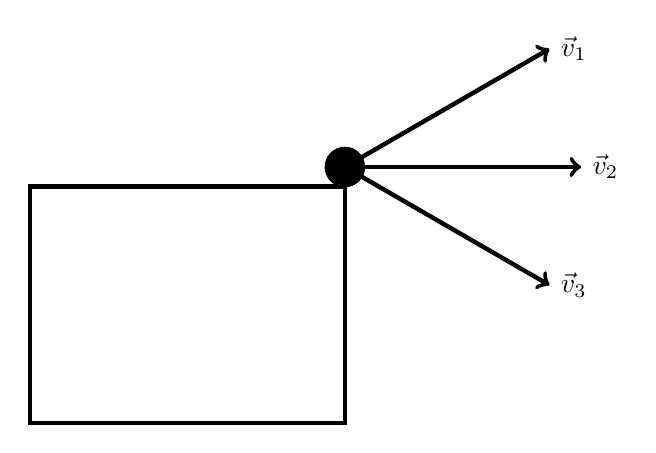
\begin{tikzpicture}
		\draw[ultra thick] (0,0) -- (4,0) -- (4,-3) -- (0,-3) -- cycle;
		\filldraw (4,0.25) circle (0.25);
		\begin{scope}[shift={(4,0.25)}]
			\draw[ultra thick,->,rotate=30] (0,0) -- (3,0) node[anchor=west] {$\vec{v}_{1}$};
			\draw[ultra thick,->] (0,0) -- (3,0) node[anchor=west] {$\vec{v}_{2}$};
			\draw[ultra thick,->,rotate=-30] (0,0) -- (3,0) node[anchor=west] {$\vec{v}_{3}$};
		\end{scope}
	\end{tikzpicture}
\end{textblock*}\newpage
\begin{TeacherMargin}

\end{TeacherMargin}
\begin{PresentSpace}
\vspace{-10pt}
\section*{Projectile Motion}
\vspace{-10pt}
\begin{itemize}
	\item Acceleration in the $x$-direction is equal to zero.
	\item Acceleration in the $y$-direction is only due to gravity.
\end{itemize}
\begin{align*}
	a_{x}(t) & = 0 & a_{y}(t) & = -g \\
	v_{x}(t) & = v_{ix} & v_{y}(t) & = v_{iy} - gt \\
	x(t) & = x_{i} + v_{ix}t & y(t) & = y_{i} + v_{iy}t -\frac{1}{2}gt^{2}
\end{align*}
\end{PresentSpace}
\newpage
\begin{TeacherMargin}

\end{TeacherMargin}
\begin{PresentSpace}
\vspace{-10pt}
\section*{Three Marbles}
\vspace{-10pt}
\begin{itemize}
	\item You throw three marbles off a table, each with the \\
	same initial speed, but in a different direction.
	\begin{itemize}
		\item Which is in the air for \\
		the most time?
		\item Which travels the most \\
		horizontal distance?
		\item Which is moving fastest \\
		when it hits?
	\end{itemize}
\end{itemize}
\end{PresentSpace}
\begin{textblock*}{10cm}(18.5cm,1.5cm)
\Large
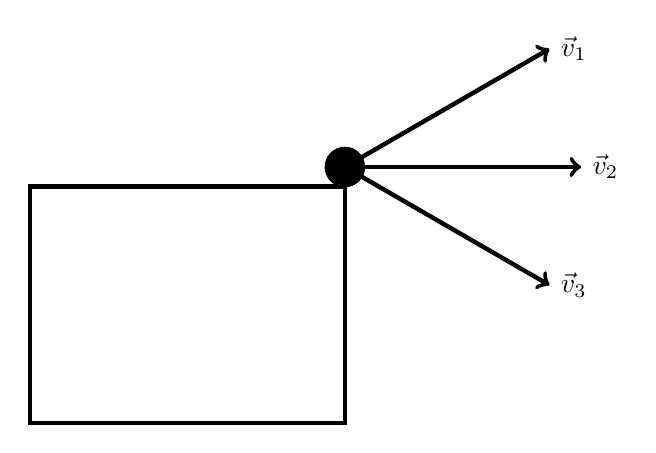
\begin{tikzpicture}
	\draw[ultra thick] (0,0) -- (4,0) -- (4,-3) -- (0,-3) -- cycle;
	\filldraw (4,0.25) circle (0.25);
	\begin{scope}[shift={(4,0.25)}]
		\draw[ultra thick,->,rotate=30] (0,0) -- (3,0) node[anchor=west] {$\vec{v}_{1}$};
		\draw[ultra thick,->] (0,0) -- (3,0) node[anchor=west] {$\vec{v}_{2}$};
		\draw[ultra thick,->,rotate=-30] (0,0) -- (3,0) node[anchor=west] {$\vec{v}_{3}$};
	\end{scope}
\end{tikzpicture}
\end{textblock*}
\newpage
\begin{TeacherMargin}
\begin{center}
	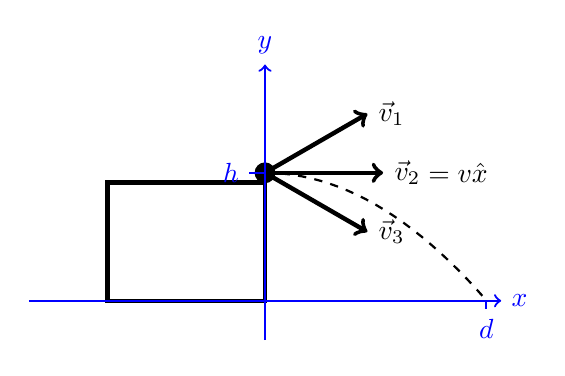
\begin{tikzpicture}
		\draw[ultra thick] (0,0) -- (2,0) -- (2,-1.5) -- (0,-1.5) -- cycle;
		\filldraw (2,0.125) circle (0.125);
		\begin{scope}[shift={(2,0.125)}]
			\draw[ultra thick,->,rotate=30] (0,0) -- (1.5,0) node[anchor=west] {$\vec{v}_{1}$};
			\draw[ultra thick,->] (0,0) -- (1.5,0) node[anchor=west] {$\vec{v}_{2}$};
			\draw[ultra thick,->,rotate=-30] (0,0) -- (1.5,0) node[anchor=west] {$\vec{v}_{3}$};
		\end{scope}
		\begin{comment}%Marble 1
			\draw[blue,thick,->] (-1,-1.5) -- (8,-1.5) node[anchor=west] {$x$};
			\draw[thick,dashed,domain=0:5,variable=\x] plot ({\x+2},{0.125+0.7*\x-0.205*\x*\x});
			\draw[blue,thick] (7,-1.5) -- (7,-1.6) node[anchor=north] {$d$};
			\draw[thick] (2.5,0.125) node[anchor=south west,shift={(0,-1pt)}] {$\theta$} arc (0:30:0.5);
			\node[anchor=west] at (5,1) {$\vec{v}_{1} = v\cos\theta\hat{x}+v\sin\theta\hat{y}$};
		\end{comment}
		\begin{scope}%Marble 2
			\draw[blue,thick,->] (-1,-1.5) -- (5,-1.5) node[anchor=west] {$x$};
			\draw[thick,dashed,domain=0:2.81,variable=\x] plot ({\x+2},{0.125-0.205*\x*\x});
			\draw[blue,thick] (4.81,-1.5) -- (4.81,-1.6) node[anchor=north] {$d$};
			\node[anchor=west] at (3.95,0.125) {$ = v\hat{x}$};
		\end{scope}
		\draw[blue,thick,->] (2,-2) -- (2,1.5) node[anchor=south] {$y$};
		\draw[blue,thick] (2,0.125) -- (1.8,0.125) node[anchor=east] {$h$};
	\end{tikzpicture}
\end{center}
To find the final time with the given information, it makes sense to use the position kinematics equations:
\begin{align*}
	x(t) & = vt & y(t) & = h - \frac{1}{2}gt^{2}
\end{align*}
\begin{multicols}{2}
	The time of flight can be determined based on how far the marble has to fall.
	\begin{align*}
		0 = y(t_{f}) & = h - \frac{1}{2}gt_{f}^{2} \\
		\frac{1}{2}gt_{f}^{2} & = h \\
		t_{f} & = \sqrt{2\frac{h}{g}}
	\end{align*}
	The horizontal distance traveled can then be determined using this time.
	\begin{align*}
		d = x(t_{f}) & = vt_{f} \\
		d = v\sqrt{2\frac{h}{g}}
	\end{align*}
\end{multicols}
\begin{multicols}{2}
\noindent We know $v_{x}(t) = v$, so $v_{fx} = v$. We also know
\begin{align*}
	v_{fy} = -gt_{f} = -g\sqrt{2\frac{h}{g}} = -\sqrt{2gh}.
\end{align*}
Therefore, the final speed is
\begin{align*}
	v_{f} & = \sqrt{v_{fx}^{2}+v_{fy}^{2}} \\
	& = \sqrt{v^{2}+2gh}.
\end{align*}
\end{multicols}
\end{TeacherMargin}
\begin{PresentSpace}
\vspace{-10pt}
\section*{S3-1: Marble 2}
\vspace{-10pt}
\begin{itemize}
	\item You throw three marbles off a table, each with the \\
	same initial speed, but in a different direction.
	\vspace{10pt}
	\begin{itemize}
		\item If the height of the table \\
		is $h$, how much time does \\
		it take for marble 2 to hit \\
		the ground?
		\item How far has the marble \\
		traveled horizontally in that amount of time?
		\item What is the marble's speed when it hits the ground?
	\end{itemize}
\end{itemize}
\end{PresentSpace}
\begin{textblock*}{10cm}(18.5cm,1.5cm)
	\Large
	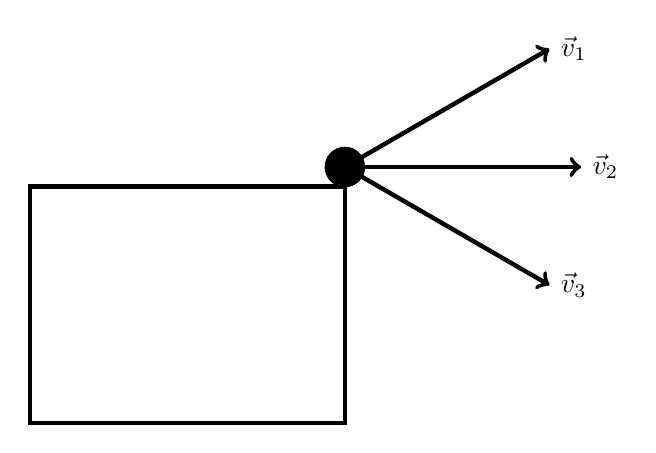
\begin{tikzpicture}
		\draw[ultra thick] (0,0) -- (4,0) -- (4,-3) -- (0,-3) -- cycle;
		\filldraw (4,0.25) circle (0.25);
		\begin{scope}[shift={(4,0.25)}]
			\draw[ultra thick,->,rotate=30] (0,0) -- (3,0) node[anchor=west] {$\vec{v}_{1}$};
			\draw[ultra thick,->] (0,0) -- (3,0) node[anchor=west] {$\vec{v}_{2}$};
			\draw[ultra thick,->,rotate=-30] (0,0) -- (3,0) node[anchor=west] {$\vec{v}_{3}$};
		\end{scope}
	\end{tikzpicture}
\end{textblock*}
\newpage
\begin{TeacherMargin}
\begin{center}
	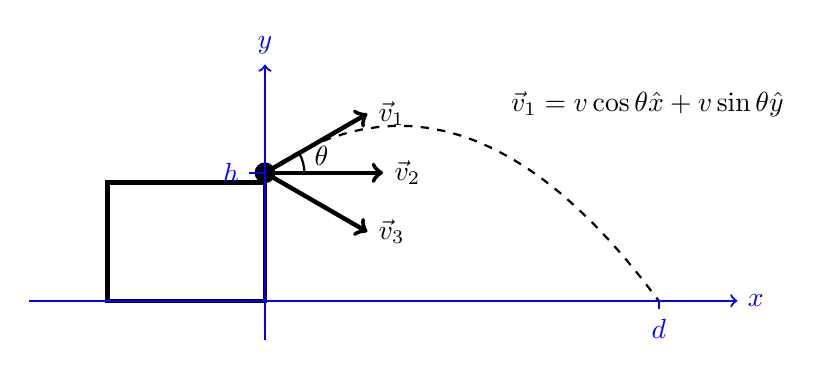
\begin{tikzpicture}
		\draw[ultra thick] (0,0) -- (2,0) -- (2,-1.5) -- (0,-1.5) -- cycle;
		\filldraw (2,0.125) circle (0.125);
		\begin{scope}[shift={(2,0.125)}]
			\draw[ultra thick,->,rotate=30] (0,0) -- (1.5,0) node[anchor=west] {$\vec{v}_{1}$};
			\draw[ultra thick,->] (0,0) -- (1.5,0) node[anchor=west] {$\vec{v}_{2}$};
			\draw[ultra thick,->,rotate=-30] (0,0) -- (1.5,0) node[anchor=west] {$\vec{v}_{3}$};
		\end{scope}
		\begin{scope}%Marble 1
			\draw[blue,thick,->] (-1,-1.5) -- (8,-1.5) node[anchor=west] {$x$};
			\draw[thick,dashed,domain=0:5,variable=\x] plot ({\x+2},{0.125+0.7*\x-0.205*\x*\x});
			\draw[blue,thick] (7,-1.5) -- (7,-1.6) node[anchor=north] {$d$};
			\draw[thick] (2.5,0.125) node[anchor=south west,shift={(0,-1pt)}] {$\theta$} arc (0:30:0.5);
			\node[anchor=west] at (5,1) {$\vec{v}_{1} = v\cos\theta\hat{x}+v\sin\theta\hat{y}$};
		\end{scope}
		\begin{comment}%Marble 2
			\draw[blue,thick,->] (-1,-1.5) -- (5,-1.5) node[anchor=west] {$x$};
			\draw[thick,dashed,domain=0:2.81,variable=\x] plot ({\x+2},{0.125-0.205*\x*\x});
			\draw[blue,thick] (4.81,-1.5) -- (4.81,-1.6) node[anchor=north] {$d$};
			\node[anchor=west] at (3.95,0.125) {$ = v\hat{x}$};
		\end{comment}
		\draw[blue,thick,->] (2,-2) -- (2,1.5) node[anchor=south] {$y$};
		\draw[blue,thick] (2,0.125) -- (1.8,0.125) node[anchor=east] {$h$};
	\end{tikzpicture}
\end{center}
We use the same starting place as before, albeit with more complicated terms:
\begin{align*}
x(t) & = v\cos\theta t, & y(t) & = h + v\sin\theta t - \frac{1}{2}gt^{2}.
\end{align*}
%\begin{multicols}{2}
The time of flight can be determined based on how far the marble has to fall. This time, we need the quadratic formula:
\begin{align*}
	0 = y(t_{f}) & = h + v\sin\theta t_{f} - \frac{1}{2}gt_{f}^{2} \\
	t_{f} & = \frac{-v\sin\theta \pm \sqrt{v^{2}\sin^{2}\theta + 4\cdot\frac{1}{2}g\cdot h}}{-g} \\
	t_{f} & = \frac{v}{g}\sin\theta \mp \sqrt{\frac{v^{2}}{g^{2}}\sin^{2}\theta + 2\frac{h}{g}}
\end{align*}
Which sign do we use? Note that $\sqrt{\frac{v^{2}}{g^{2}}\sin^{2}\theta + 2\frac{h}{g}} \geq |\frac{v}{g}\sin\theta|$, and $t_{f}$ occurs in the future, so we need to pick the sign that keeps the expression positive (a negative time does have a physical interpretation; this is the time the marble would have started at to undergo this motion, had it been launched from the ground). As such, we want to use $+$, as it is the only way to make $t_{f}$ positive:
\begin{align*}
	t_{f} = \frac{v}{g}\sin\theta + \sqrt{\frac{v^{2}}{g^{2}}\sin^{2}\theta + 2\frac{h}{g}}.
\end{align*}
\noindent The distance traveled is just $d = v\cos\theta t_{f}$, so the above expression can be plugged in. The final speed is much more interesting:
\begin{align*}
	v_{fx} & = v_{ix} = v\cos\theta & v_{fy} & = v\sin\theta - gt_{f} \\
	& & & = v\sin\theta - g \left[\frac{v}{g}\sin\theta + \sqrt{\frac{v^{2}}{g^{2}}\sin^{2}\theta + 2\frac{h}{g}}\right] \\
	& & & = - \sqrt{v^{2}\sin^{2}\theta + 2gh} \\
\end{align*}
\vspace{-1cm}
\begin{align*}
	v_{f} = \sqrt{v_{fx}^{2}+v_{fy}^{2}} & = \sqrt{v^{2}\cos^{2}\theta + v^{2}\sin^{2}\theta+2gh} \\
	& = \sqrt{v^{2}\left(\cos^{2}\theta + \sin^{2}\theta\right)+2gh} = \sqrt{v^{2}+2gh}
\end{align*}
Final speed is independent of the angle! \\
\noindent We also got marble 3 for free! Just plug in a negative quantity for $\theta$.
\end{TeacherMargin}
\begin{PresentSpace}
\vspace{-10pt}
\section*{S3-2: Marble 1}
\vspace{-10pt}
\begin{itemize}
	\item You throw three marbles off a table, each with the \\
	same initial speed, but in a different direction.
	\vspace{10pt}
	\begin{itemize}
		\item If the angle is $\theta$, how \\
		long does it take for \\
		marble 1 to hit the \\
		ground?
		\item How far has the marble \\
		traveled horizontally in that amount of time?
		\item What is the marble's speed when it hits the ground?
	\end{itemize}
\end{itemize}
\end{PresentSpace}
\begin{textblock*}{10cm}(18.5cm,1.5cm)
	\Large
	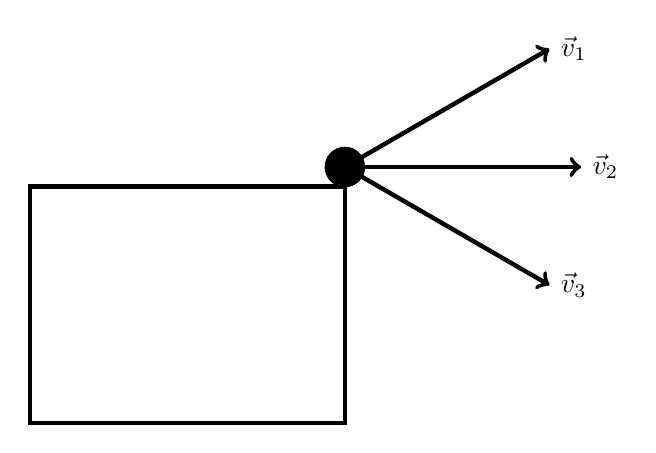
\begin{tikzpicture}
		\draw[ultra thick] (0,0) -- (4,0) -- (4,-3) -- (0,-3) -- cycle;
		\filldraw (4,0.25) circle (0.25);
		\begin{scope}[shift={(4,0.25)}]
			\draw[ultra thick,->,rotate=30] (0,0) -- (3,0) node[anchor=west] {$\vec{v}_{1}$};
			\draw[ultra thick,->] (0,0) -- (3,0) node[anchor=west] {$\vec{v}_{2}$};
			\draw[ultra thick,->,rotate=-30] (0,0) -- (3,0) node[anchor=west] {$\vec{v}_{3}$};
		\end{scope}
	\end{tikzpicture}
\end{textblock*}
\newpage
\begin{TeacherMargin}
\begin{align*}
	d & = v\cos\theta \left(\frac{v}{g}\sin\theta + \sqrt{\frac{v^{2}}{g^{2}}\sin^{2}\theta+\frac{2h}{g}}\right) \\
	& = \frac{v^{2}}{g}\cos\theta\sin\theta + \sqrt{\frac{v^{4}}{g^{2}}\cos^{2}\theta\sin^{2}\theta+\frac{2hv^{2}}{g}\cos^{2}\theta} \\
	& = \frac{v^{2}}{2g}\sin(2\theta) + \sqrt{\frac{v^{4}}{4g^{2}}\sin^{2}(2\theta)+\frac{2hv^{2}}{g}\cos^{2}\theta}
\end{align*}
\begin{center}
	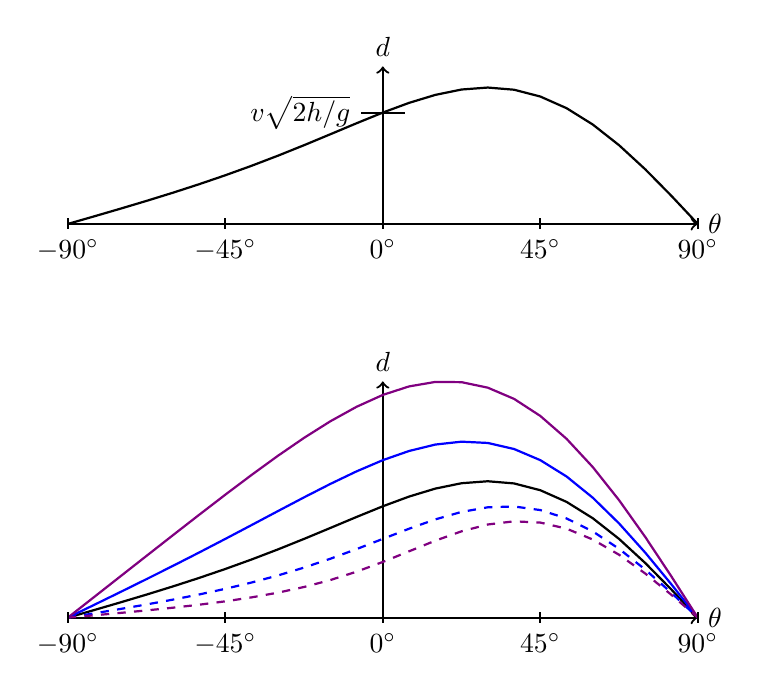
\begin{tikzpicture}
		\begin{scope}
			\draw[thick,<->] (0,2) node[anchor=south] {$d$} -- (0,0) -- (-4,0) -- (4,0) node[anchor=west] {$\theta$};
			\draw[thick,domain=-90:90,variable=\th] plot (4*\th/90,{sin(2*\th)/2 + sqrt(sin(2*\th)*sin(2*\th)/4 + 2*cos(\th)*cos(\th))});
			\foreach \th in {-90,-45,0,45,90}
				\draw[thick] ({2*\th/45},2pt) -- ({2*\th/45},-2pt) node[anchor=north] {$\th^{\circ}$};
			\draw[thick] (8pt,1.41) -- (-8pt,1.41) node[anchor=east] {$v\sqrt{2h/g}$};
		\end{scope}
		\begin{scope}[shift={(0,-5)}]
			\draw[thick,<->] (0,3) node[anchor=south] {$d$} -- (0,0) -- (-4,0) -- (4,0) node[anchor=west] {$\theta$};
			\draw[thick,domain=-90:90,variable=\th] plot (4*\th/90,{sin(2*\th)/2 + sqrt(sin(2*\th)*sin(2*\th)/4 + 2*cos(\th)*cos(\th))});
			\draw[blue,thick,domain=-90:90,variable=\th] plot (4*\th/90,{sin(2*\th)/2 + sqrt(sin(2*\th)*sin(2*\th)/4 + 4*cos(\th)*cos(\th))});
			\draw[violet,thick,domain=-90:90,variable=\th] plot (4*\th/90,{sin(2*\th)/2 + sqrt(sin(2*\th)*sin(2*\th)/4 + 8*cos(\th)*cos(\th))});
			\draw[blue,dashed,thick,domain=-90:90,variable=\th] plot (4*\th/90,{sin(2*\th)/2 + sqrt(sin(2*\th)*sin(2*\th)/4 + 1*cos(\th)*cos(\th))});
			\draw[violet,dashed,thick,domain=-90:90,variable=\th] plot (4*\th/90,{sin(2*\th)/2 + sqrt(sin(2*\th)*sin(2*\th)/4 + cos(\th)*cos(\th)/2)});
			\foreach \th in {-90,-45,0,45,90}
				\draw[thick] ({2*\th/45},2pt) -- ({2*\th/45},-2pt) node[anchor=north] {$\th^{\circ}$};
		\end{scope}
	\end{tikzpicture}
\end{center}
Each curve shows the distance $d$ as a function of the launch angle $\theta$. These plots assumed that $v = 1$ m/s and $g = 1$ m/s$^{2}$. The black curve is for $h=1$ m, while the solid blue and purple curves are for $h=2$ m and $h=4$ m, respectively, and the dashed blue and purple curves are for $h=0.5$ m and $h=0.25$ m, respectively. The distance always increases with increasing $h$, but the angle $\theta_{\text{max}}$ at which the maximum distance occurs decreases with increasing $h$.

It appears that, as $h$ decreases, $\theta_{\text{max}}$ approaches 45$^{\circ}$, which is the angle for maximum range when the projectile starts and ends at the same height.
\end{TeacherMargin}
\begin{PresentSpace}
\vspace{-10pt}
\section*{Three Marbles}
\vspace{-10pt}
\begin{itemize}
	\item You throw three marbles off a table, each with the \\
	same initial speed, but in a different direction.
	\vspace{1cm}
	\begin{itemize}
		\item If $h$ is the height of the \\
		table, $v$ is the initial \\
		speed, and $\theta$ is the angle \\
		up from the horizontal:
	\end{itemize}
\end{itemize}
\begin{align*}
	t_{f} & = \frac{v}{g}\sin\theta + \sqrt{\frac{v^{2}}{g^{2}}\sin^{2}\theta+\frac{2h}{g}} & d & = vt_{f}\cos\theta & v_{f} & = \sqrt{v^{2}+2gh}
\end{align*}
\end{PresentSpace}
\begin{textblock*}{10cm}(18.5cm,1.5cm)
	\Large
	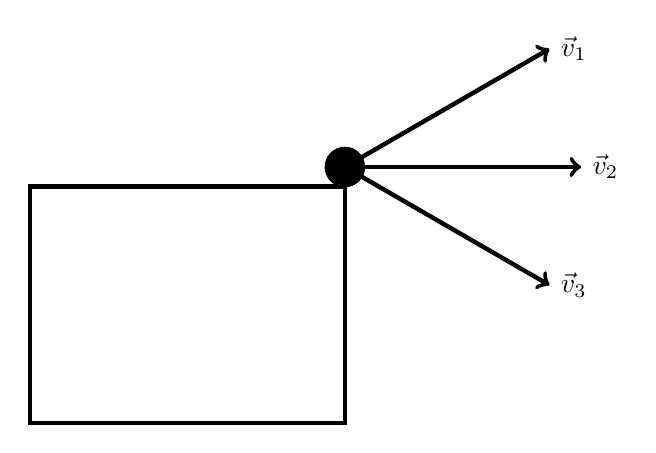
\begin{tikzpicture}
		\draw[ultra thick] (0,0) -- (4,0) -- (4,-3) -- (0,-3) -- cycle;
		\filldraw (4,0.25) circle (0.25);
		\begin{scope}[shift={(4,0.25)}]
			\draw[ultra thick,->,rotate=30] (0,0) -- (3,0) node[anchor=west] {$\vec{v}_{1}$};
			\draw[ultra thick,->] (0,0) -- (3,0) node[anchor=west] {$\vec{v}_{2}$};
			\draw[ultra thick,->,rotate=-30] (0,0) -- (3,0) node[anchor=west] {$\vec{v}_{3}$};
		\end{scope}
	\end{tikzpicture}
\end{textblock*}
\newpage
\begin{TeacherMargin}
\begin{itemize}
	\item What does it mean to say that two objects are interacting?
	\begin{itemize}
		\item We will be characterizing interactions in terms of forces between objects, which is to say we are looking at how objects push and pull each other.
	\end{itemize}
	\item What happens to objects when they interact?
	\begin{itemize}
		\item Interacting objects affect each other's motion. Objects that do not interact say at a constant velocity, while interacting objects may accelerate.
	\end{itemize}
	\item What if multiple objects interact with the same object?
	\begin{itemize}
		\item We associate each force with a pair of interacting objects, so we account for (at least) one force for each object interacting with the object of interest. All of these forces are added together (as vectors) to find the net force on the object of interest.
	\end{itemize}
\end{itemize}
\end{TeacherMargin}
\begin{PresentSpace}
\vspace{-10pt}
\section*{What are Interactions/Forces?}
\vspace{-10pt}
\begin{itemize}
	\item What does it mean to say that two objects are interacting?
	\item What happens to objects when they interact?
	\item What if multiple objects interact with the same object?
	\item \textbf{What different kinds of interactions are there?}
\end{itemize}
\end{PresentSpace}
\newpage
\begin{TeacherMargin}
\noindent\textbf{This Week:} Gravity and Normal Force \\
\textbf{Next Week:} Friction (kinetic and static), Tension, and Springs \\
\textbf{PH 213:} Electric and Magnetic Force
\end{TeacherMargin}
\begin{PresentSpace}
\vspace{-10pt}
\section*{Types of Forces}
\vspace{-10pt}
\begin{itemize}
	\item Gravity: $\vec{F}^{g}$
	\item Normal: $\vec{F}^{N}$
	\item Tension: $\vec{F}^{T}$
	\item Spring: $\vec{F}^{sp}$
	\item Friction: $\vec{F}^{f}$ ($\vec{F}^{kf}$, $\vec{F}^{sf}$)
	\item Electric: $\vec{F}^{E}$
	\item Magnetic: $\vec{F}^{M}$
\end{itemize}
\end{PresentSpace}
\newpage
\begin{TeacherMargin}

\end{TeacherMargin}
\begin{PresentSpace}
\vspace{-10pt}
\section*{Normal Forces}
\vspace{-10pt}
\begin{itemize}
	\item Normal forces are contact forces that act perpendicular to the surface of contact.
	\item There is no formula for determining normal forces---the magnitude can change
	depending on the circumstances.
	\item Too much normal force can cause objects to break!
\end{itemize}
\end{PresentSpace}
\newpage
\begin{TeacherMargin}

\end{TeacherMargin}
\begin{PresentSpace}
\vspace{-10pt}
\section*{Tension Forces}
\vspace{-10pt}
\begin{itemize}
	\item Tension forces are kind of like normal forces, except they pull in the direction of
	the rope.
	\item There is no formula for determining tension forces---the magnitude can change depending on the circumstances.
	\item Too much tension force can cause a rope to break!
	\item Tension is uniform throughout a single rope.
	\begin{itemize}
		\normalsize
		\item \dots if the rope is massless, inextensible, and the middle of the rope isn’t in contact with anything.
	\end{itemize}
\end{itemize}
\end{PresentSpace}
\newpage
\begin{TeacherMargin}

\end{TeacherMargin}
\begin{PresentSpace}
\vspace{-10pt}
\section*{Free-Body Diagrams and Systems}
\vspace{-10pt}
\begin{itemize}
	\item Choose a system.
	\begin{itemize}
		\large
		\item Make sure you know what is internal to your system and what is external to your system.
	\end{itemize}
	\item Identify and describe each external force:
	\begin{itemize}
		\large
		\item Say what kind of force it is.
		\item Determine the object the force is being acted on.
		\item Determine the object that is exerting the force.
		\item Write a symbolic version of the force that includes the information above.
		\item Represent all the forces acting on a single object or system using a \\
		\textbf{\underline{free-body diagram}}.
	\end{itemize}
\end{itemize}
\end{PresentSpace}
\begin{textblock*}{5cm}(22cm,3.5cm)
	\Huge
	\[
	\vec{F}^{\text{\Large\ type}}_{\text{\Large on,by}}
	\]
\end{textblock*}
\newpage
\begin{TeacherMargin}
\noindent In all three cases, there are two forces acting on the bag of groceries:
\begin{itemize}
	\item $\vec{F}^{N}_{BH} = F^{N}\hat{y}$: normal force of the hand pushing up on the bag.
	\item $\vec{F}^{g}_{BE} = F^{g}(-\hat{y})$: gravitational force of Earth pulling down on the bag.
\end{itemize}
In cases (A) and (C), the forces are equal in magnitude, as the motion of the bag is not changing. In (B), the bag is accelerating downward, so the normal force must be smaller than the gravitational force. \\
\noindent\textbf{(A)} \\
There isn't really a motion diagram in this case, as the bag is not moving.
\begin{center}
	\begin{tikzpicture}
		\draw[thick] (-0.5,-0.5) -- (0,0) -- (0.5,-0.5) (0,0) -- (0,1) (-0.5,0.5) -- (0,1) -- (0.75,1) (0,1.3) circle (0.3) (0.6,1.05) rectangle (0.9,1.65);
		\filldraw (2,1.35) circle (2pt);
		\FBDaxes[1.5]{4.5,0.5}{0}{axes}
		\FBDvectorXY{axes}{0,1}{FN}
		\FBDvectorXY{axes}{0,-1}{FG}
		\FBDdot{axes}
	\end{tikzpicture}
\end{center}
\noindent\textbf{(B)}
\begin{center}
	\begin{tikzpicture}
		\draw[thick] (-0.5,-0.5) -- (0,0) -- (0.5,-0.5) (0,0) -- (0,1) (-0.5,0.5) -- (0,1) -- (0.75,1) (0,1.3) circle (0.3) (0.6,1.05) rectangle (0.9,1.65);
		\draw[thick,->] (1.1,1.65) -- (1.1,1.05);
		\node[anchor=south] at (2,1.35) {$t_{0}$};
		\foreach \t in {0,1,2,3}
			\filldraw (2,{1.35-\t*\t/5}) circle (2pt);
		\FBDaxes[1.5]{4.5,0.5}{0}{axes}
		\FBDvectorXY{axes}{0,0.65}{FN}
		\FBDvectorXY{axes}{0,-1}{FG}
		\FBDdot{axes}
	\end{tikzpicture}
\end{center}
\noindent\textbf{(C)}
\begin{center}
	\begin{tikzpicture}
		\draw[thick] (-0.5,-0.5) -- (0,0) -- (0.5,-0.5) (0,0) -- (0,1) (-0.5,0.5) -- (0,1) -- (0.75,1) (0,1.3) circle (0.3) (0.6,1.05) rectangle (0.9,1.65);
		\draw[thick,<-] (1.1,1.65) -- (1.1,1.05);
		\node[anchor=north] at (2,1.35) {$t_{0}$};
		\foreach \t in {0,1,2,3}
			\filldraw (2,{1.35+\t/3}) circle (2pt);
		\FBDaxes[1.5]{4.5,0.5}{0}{axes}
		\FBDvectorXY{axes}{0,1}{FN}
		\FBDvectorXY{axes}{0,-1}{FG}
		\FBDdot{axes}
	\end{tikzpicture}
\end{center}
\end{TeacherMargin}
\begin{PresentSpace}
\vspace{-10pt}
\section*{S3-3: The Bag of Groceries}
\vspace{-10pt}
\begin{multicols}{2}
For each situation to the right:
\begin{enumerate}[(1)]
	\item Sketch a picture of the object of interest.
	\item Make a strobe or motion diagram.
	\item Identify and describe the forces acting on the object.
	\item Draw a free-body diagram for the object.
\end{enumerate}
\begin{enumerate}[(A)]
	\item You hold a bag of groceries in your hand.
	\item You lower the bag of groceries; the bag moves downward faster and faster.
	\item You lift the bag of groceries; the bag moves upward at constant speed.
\end{enumerate}
\end{multicols}
\end{PresentSpace}
\newpage
\begin{TeacherMargin}

\end{TeacherMargin}
\begin{PresentSpace}
\section*{Main Ideas}
\begin{itemize}
	\item Motion in 2 dimensions can be broken down into independent motion in each dimension.
	\item Solving a problem symbolically allows you to solve many problems with one set of algebra.
	\item Forces arise from interactions between objects.
	\item There are many different kinds of forces that we can analyze differently.
	\item Objects can only change their motion when acted upon by an external force.
\end{itemize}
\end{PresentSpace}
\end{document}